% \chapter{Background Theory}
\chapter{\chapterTwo}
\label{chp:2}

\textit{This chapter examines some background theory related to security, cryptography, and PUF. A brief review of security is presented, followed by explanations on symmetric cryptography, key derivation function and multi-factor authentication.
Then, theories related to PUF and SRAM PUF are described, continued by a short evaluation on how to generate a key using SRAM PUF.}

\section{Security Requirements and Cryptography}
\label{chapter2.1}

A perfect and 100\% secure system is the holy grail of all computing system. Unfortunately, such thing doesn't exist. The best way to achieve that goal is by designing a system to be as secure as possible in a limited scope.
To help defining a secure system, common security requirements are mentioned.
According to \cite{cryptography_decrypted}, there are four elements on common security, which are:
\begin{itemize}
  \item \textit{Confidentiality}: a piece of information should be accessible only to an authorized user. For example, an encrypted data can only be decrypted by the secret key owner.
  \item \textit{Authentication}: assurance of the sender of a message, date of origin, data content, time sent, data information, etc. are correctly identified.
  \item \textit{Integrity}: any assets can only be modified by authorized subjects. For example, data should be kept intact during transmission
  \item \textit{Non-repudiation}: a subject should be prevented from denying previous actions. For example, a sender cannot deny the data which it sent.
\end{itemize}

One way to achieve these four security requirements is by using cryptography. In traditional definition, cryptography can be defined as the art of writing or solving codes \cite{Oxford_dictionary}. But this definition is inaccurate to use nowadays because instead of depending on creativity and personal skill when constructing or breaking codes, the modern cryptography focuses their definition using science and mathematics. According to \cite{modern_cryptography}, modern cryptography can be defined as "the scientific study of techniques for securing digital information, transactions, and distributed computations." The algorithm which uses cryptography as their main point is called cryptographic algorithm.

Since the birth of cryptography, its main concerned is usually related to securing communication which can be achieved by constructing \textit{ciphers} to provide secret communication between parties involved. The construction of ciphers to ensure only authorized parties also can be called as encryption schemes.
There are two types of cryptographic algorithm; symmetric and asymmetric algorithm. Symmetric, also known as private key encryption or private key cryptography, requires the same key for encryption and decryption. Meanwhile, in the asymmetric algorithm (can be referred as public key encryption or public key cryptography), there are two keys utilized; private key and public key. A public key is utilized for encryption and a private key is used for decryption. One of the main advantages of symmetric encryption over asymmetric encryption is it requires less computational power which makes it suitable to use in embedded devices.

\section{Symmetric Encryption}

According to \cite{modern_cryptography}, symmetric encryption consists of three algorithms which are:
\begin{itemize}
    \item \large{\textit{Gen}}: key-generation algorithm
    \item \large{\textit{Enc}}: encryption algorithm
    \item \large{\textit{Dec}}: decryption algorithm
\end{itemize}
To illustrate this better, an example using two parties, Alice and Bob are given. Before using the encryption or decryption algorithm, both parties will agree on a shared secret key $k$. This phase can be referred as \large{Gen}.
Afterwards, Alice can use the encryption algorithm (\large{Enc}) $E_k$ using the shared secret key $k$ on a message $m$ which will generates a ciphertext $c$. This procedure can be noted as $c\ =\ E_k(m)$. Bob can read the message by using the decryption algorithm (\large(Dec)) $Dec_k$ using the same shared secret key $k$. Decryption will result in the plaintext message $m$. This can be noted as $m\ =\ D_k(c)$.


There are many examples of symmetric encryption algorithms, such as RC2, DES, 3DES, RC6, Blowfish, and AES. AES algorithm will be explained below.

\subsubsection{AES}
AES, stands for Advanced Encryption Standard, is an encryption algorithm based on a substitution-permutation network and established by the U.S. National Institute of Standards and Technology (NIST) in 2001.
The block size inside AES has a size of 128 bits, while the key size can be either 128, 192, or 256 bits. The key size  itself describes the number of rounds which convert the plaintext into the ciphertext. If 128-bit key is used, there are 10 rounds utilized. 192-bit key lead to 12 rounds, while 14 rounds is used when 256-bit key is applied.


There are four major parts inside AES; \textit{KeyExpansions}, \textit{InitialRound}, \textit{Rounds} and \textit{FinalRound}. In KeyExpansions, the round keys are generated using Rijndael's key schedule based on the AES key.
Inside a normal round, there are four stages required to do; \textit{SubBytes}, \textit{ShiftRows}, \textit{MixColumns}, and \textit{AddRoundKey}.
SubBytes refers to a non-linear substitution procedure using a lookup table. ShiftRows means an act of shifting cyclically the last three rows of the state. MixColumns contains a mixing activity on the columns of the state.
AddRoundKey involves a fusing process of each byte of the state with a block of the round key utilizing bitwise xor operation. The difference between InitialRound, Rounds, and FinalRound is InitialRound only contain AddRoundKey, FinalRound does not has MixColumns inside, and Rounds just filled with those four stages.

An encryption can be done by following all these four parts. To convert ciphertext into the original plaintext, it's only required to apply a set of reverse rounds using the same encryption key.

\section{Key Derivation Function}
Besides the encryption algorithm, a \textit{key derivation function} (KDF) is one of the most utilized components of cryptographic applications. Its importance is due to its ability to convert a stable secret, usually contain sufficient amount of randomness but non-uniformly distributed,  $Z$ into one or more cryptographically strong secret keys $k\ \epsilon\ {0,1}^K$.
Cryptographically strong itself refers to indistinguishability by reasonable computation from a random uniform string with similar length \cite{key_derivation}.
KDF can also be referred as a strong extractor.

A popular example of KDF is a keyed cryptographic hash function. The difference between keyed cryptographic hash function and a normal hash function is a keyed hash function requires an additional \textit{salt} as an input (besides the key to derived).
There are three requirements need to be fulfilled as a secure cryptographic hash function; \textit{preimage resistant, second preimage resistant, and collision resistant}. Preimage resistant means it should be hard to find a message with a given hash value. In second preimage resistant, if one message is provided, it should be hard to find another message with the same hash value.
Last, collision resistant refers to difficultness to find two messages with the same hash value.

\section{Multi-factor Authentication}
\label{chp:2.mfa}
As mentioned in Section \ref{chapter2.1}, authentication refers to assuring any piece of information is correctly identified. Authentication can be done using any of these elements/factors; knowledge (a piece of information which only known by the user, e.g. password), possession (any object which only owned by the user, e.g. RFID card), or inherence (something which uniquely describe the user, e.g. fingerprint). If two or more elements are combined together for authentication, this leads to \textit{multi-factor authentication}. To understand the security level among all possible combinations, Figure \ref{fig:authentication} is provided. The highest possible security level is when these three factors are combined together.

\begin{figure}[tph!]
    \centerline{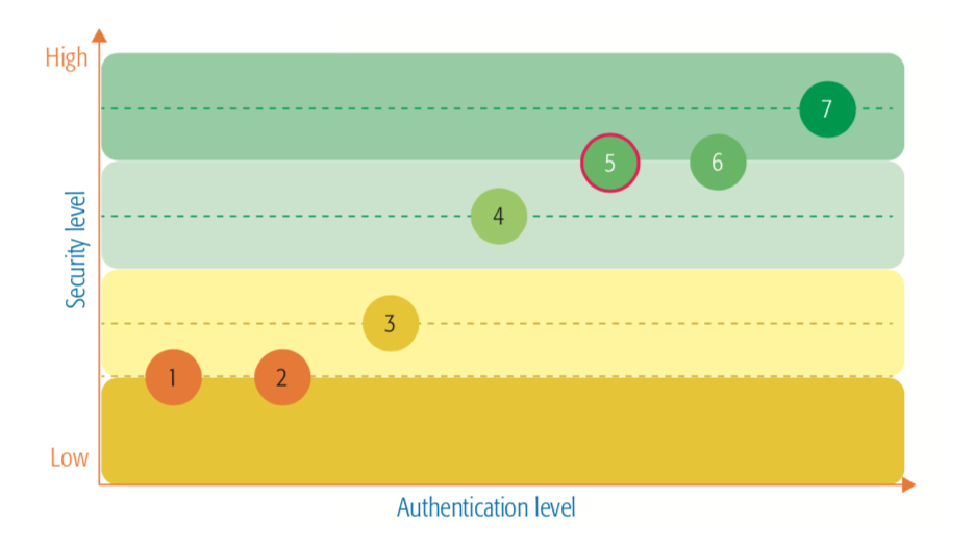
\includegraphics[width={0.5\textwidth}]{images/authentication}}
    \caption{Authentication systems security levels: (1) knowledge; (2) possession; (3) knowledge + inherence; (4) inherence; (5) possession + inherence; (6) knowledge + inherence; (7) knowledge + possesion + inherence \cite{Galdi2018ExploringNA}.}
    \label{fig:authentication}
\end{figure}


\section{PUF}
A physical unclonable function is an entity that utilizes manufacturing variability to produce a device-specific output. The idea to build PUF arise from the fact that even though the mask and manufacturing process is the same among different ICs, each IC is actually slightly different due to normal manufacturing variability \cite{retrospective}. PUFs leverage this variability to derive secret information that is unique to the chip. This secret can be referred as a silicon biometric.
In addition, due to the manufacturing variability that defines the secret, one cannot manufacture two identical chips, even with full knowledge of the chip’s design. PUF architectures exploit manufacturing variability in multiple ways. For example, one can utilize the effect of gate delay, the power-on state of SRAM, threshold voltages, and many other physical characteristics to derive the secret.

Due to this feature, PUFs are a promising innovative primitive that is used for authentication and secret key storage without the requirement of secure hardware. Currently, the best practice for providing a secure memory or authentication source in such a mobile system is to place a secret key in a nonvolatile electrically erasable programmable read-only memory (EEPROM) or battery-backed static random-access memory (SRAM) and use hardware cryptographic operations such as digital signatures or encryption.

There are two main parts of PUF, physical part, and operational part. Physical part refers to a physical system that is very difficult to clone due to uncontrollable process variations during manufacturing. Operational part means a set of \textit{challenges} (PUF input) $C_i$ has to be available to which the system responds with a set of sufficiently different \textit{responses} (PUF output) $R_i$. This combination of challenge and response is called \textit{challenge-response-pair} (CRP).
\begin{equation}
R_i <- PUF(C_i)
\end{equation}

The common application on using PUF usually requires two phases; the first phase is called \textit{enrollment} and the second one is usually referred as \textit{validation}. In enrollment, a number of CRPs are gathered from a PUF and then stored. In validation phase, a challenge from the stored CRPs is given to the PUF. Afterwards, the PUF response from this challenge is compared with the corresponding response from the database. The response is considered to be valid if there's a CRP from the stored CRPs related to this challenge and response. The validation phase can also be referred as \textit{reproduction} phase since this phase involves a reconstruction of a response given a challenge.

According to \cite{retrospective}, to be qualified as PUF, a device should fulfill several characteristics below :
\begin{itemize}
\item \textit{Reliable}: A response to the same challenge should be able to be reproduced over time and over a various range of conditions.
\item \textit{Unpredictable}: A response to a challenge on a PUF device should be unrelated to a response to another challenge from the same device or the same challenge from a different device.
\item \textit{Unclonable}: Challenge-response pairs mapping of a device should be unique and cannot be duplicated.
\item \textit{Physically Unbreakable}: Any physical attempts to maliciously modify the device will result in malfunction or permanent damage.
\end{itemize}

\subsection{PUFs Classification} \label{lbl:puf-classification}

Based on the number CRPs, PUFs can be divided into two categories \cite{Srivathsa2017SecureAE}:
\begin{itemize}
\item Strong PUFs\newline
Strong PUFs can be identified by having a large number of CRPs. Strong PUFs typically used for authentication.
\item Weak PUFs\newline
Contrary to strong PUFs, weak PUFs only have a small number of CRPs. Weak PUFs commonly used for key storage.
\end{itemize}

Besides the number of CRPs, PUFs can also be categorized based on their physical design. There are two major categories, extrinsic and intrinsic.

Extrinsic means that it needs extra hardware added to the PUF component. The extra hardware is required to access the PUF component. There are two subcategories of extrinsic PUFs, non-electronic and analog electronic PUFs. Some examples in non-electronic PUFs are optical PUF, paper PUF, CD PUF, RF-DNA PUF, magnetic PUF, and acoustic PUF. Some design instances in analog electronic PUFs are VT PUF, power distribution PUF, coating PUF, and LC PUF.

In intrinsic, the PUF component has to be available naturally during the manufacturing process. In addition, PUF and the measurement equipment should be fully integrated with intrinsic PUF. There are two subcategories in intrinsic PUFs, delay based and memory based PUFs. An example of delay based PUF is arbiter PUF. The main principle of arbiter PUF is by presenting a race condition on two different routes on a chip where the winner will be decided by an arbiter circuit \cite{study_of_the_art_puf}. As in memory based PUFs, some examples of this design are SRAM PUF, butterfly PUF and latch PUF. SRAM PUF utilized the random physical mismatch in the cell introduced by manufacturing variability which controls the power-up behavior (can be zero, one, or no preference) \cite{study_of_the_art_puf}. Butterfly PUF use the effect of cross coupling between two transparent data latches. Using the functionalities of the latches, an unsteady condition can be initiated after which the circuit resolves back to one of the two stable states \cite{study_of_the_art_puf}. In latch PUF, the concept is based on using two NOR gates which are cross-coupled. These gates will lead to a stable condition depending on the internal discrepancy between the electronic components.

\subsection{Hamming Distances as an Identification Helper}

As explained before, PUF main purpose is dedicated for identification, shown by having a device-specific output. In PUF, \textit{hamming distance} is commonly used as a way to help defining this idea. Hamming distance itself is the number of positions at which the corresponding symbols are different on two equal length strings \cite{hamming_distance}.
There are two types of hamming distance utilized, intra-chip and inter-chip hamming distance. Inter-chip hamming distance is the distance between two responses resulting from giving a similar challenge to two distinct PUF devices \cite{study_of_the_art_puf}. Intra-chip hamming distance refers to the difference between the two responses resulting from applying a challenge twice to a PUF device \cite{modeling_sram}. To ease the identification purpose, fractional hamming distance is also introduced. Fractional hamming distance is the number of differences between two strings divided by the length of the bit strings.
In ideal PUFs, the intra-chip fractional hamming distance (HD\textsubscript{intra}) is 0\% and inter-chip fractional hamming distance (HD\textsubscript{inter}) is 50\%. Due to noises, normally PUF devices has HD\textsubscript{intra} $\leq$ 10\% and HD\textsubscript{inter} ~50\%. The identification goal will not be achieved if there is an overlap between HD\textsubscript{intra} and HD\textsubscript{inter} \cite{impact_aging}. Overlap will happen if the HD\textsubscript{intra} is too large and HD\textsubscript{inter} is too small, e.g. HD\textsubscript{intra} is 35\% and HD\textsubscript{inter} is 30\%.

\subsection{Helper Data Algorithms and Fuzzy Extractor}

There are two issues if PUF raw responses are used as a key in cryptographic primitive. First, both weak and strong PUFs rely on analog physical properties of the fabricated circuit to derive secret information. Naturally, these analog properties have noise and variability associated with them.
This can be a problem due to sensitivity of cryptographic functions on noises of their inputs.
Another issue is the PUF raw responses usually are not uniformly distributed, which makes it an unqualified as a cryptographically secure key. These two issues can be solved using \textit{Helper Data Algorithm} (HDA). One can also refer Helper Data Algorithm as \textit{fuzzy extractor} since both are capable of converting noisy information into keys usable for any cryptographic application \cite{efficient_helper} \cite{fuzzy_extractor}.

Fuzzy extractor solves both issues mentioned above by using two phases, \textit{information reconciliation} and \textit{privacy amplification}. In information reconciliation phase, possible bit errors are corrected to form a robust bit string \cite{soft_decision}. Information reconciliation is tightly related to error correction. In fact, a procedure to do information reconciliation based on error-correcting codes is called code-offset technique \cite{fuzzy_extractor}. Using code-offset technique, one should be able to reconstruct a bit string \textit{w} from a noisy version \textit{w'} as long as the Hamming distance between \textit{w}and \textit{w'} is limited to \textit{t}.
The second phase, privacy amplification, is a process to evolve this robust bit string into a full entropy key. Privacy amplification, also can be called as randomness extraction \cite{information_reconciliation}, can be done by utilizing two-way hash function.

Beside these two phases, fuzzy extractor also consists of two procedures, \large{Gen} and \large{Rep}. \large{Gen}, stands for \textit{generation}, is a probabilistic procedure which outputs an "extracted" string / key (secret) $R$ and a string (public) \textit{helper data} $P$ on input fuzzy data $w$. \large{Rep}, stands for \textit{reproduction}, is a deterministic function capable of recovering secret key $R$ from the string \textit{helper data} $P$ and any vector $w'$ as long as the Hamming distance between \textit{w}and \textit{w'} is limited to \textit{t}.
In \cite{stable_key_generation}, Taniguchi et. al illustrated the generation and reproduction procedure of fuzzy extractor on PUF which is shown in Figure \ref{fig:scheme-key-generator}.

\begin{figure}[tph!]
    \centerline{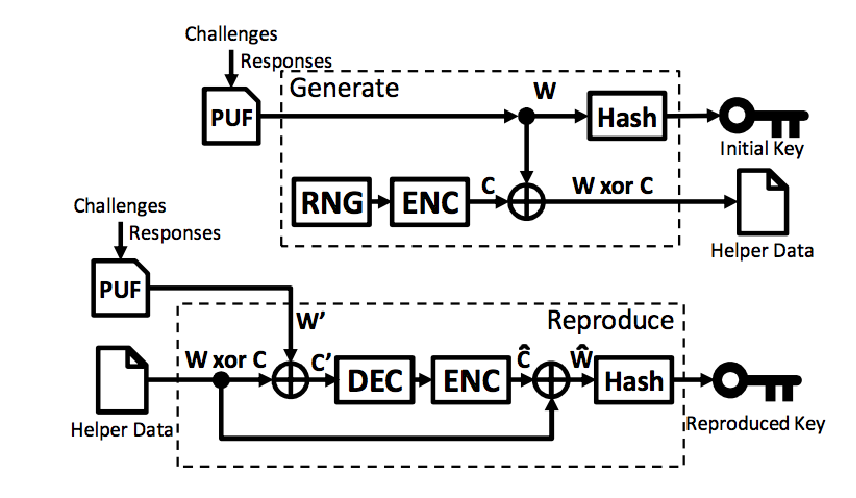
\includegraphics[width={0.8\textwidth}]{images/scheme_stable_key_generation}}
    \caption{Two procedures inside fuzzy extractor; generation and reproduction \cite{stable_key_generation}.}
    \label{fig:scheme-key-generator}
\end{figure}

\subsection{Error Correcting Codes}
To handle noises occurred inside a PUF, error-correcting codes (ECC) is employed.
Error-correcting codes are a class of schemes for encoding messages in an attempt to enable message recovery when there is noise introduced in the sending or receiving of the message. ECC can be divided into two subcategories, hard-decision and soft-decision. Hard-decision works on a predetermined set of values (usually 0 or 1 in a binary code), while a soft-decision decoder may take inputs on a span of values in-between (usually refers to float value).

There are some well-known ECC, such as in hard-decision code, Reed-Solomon code and BCH code; while in soft-decision, Viterbi code and turbo code. Soft-decision code has an advantage over hard-decision code where it can process extra information which indicates the reliability of each input data point and used to form better estimates of the original data. But it has drawback where one should provide a probability function on the data (on SRAM, a probability function on each cell should be provided) to enable a good decoding result. This is a problem if applied on this thesis goal where the system should work on any SRAM off-the-market. Calculating the probability on each SRAM cell will take an extra step, overcomplicate the system and the procedure on using the constructed system. Thus, the hard-decision code is preferred.

One of the popular hard-decision error correcting code is BCH codes. BCH, stands for \textit{Bose–Chaudhuri–Hocquenghem}, codes are a family of cyclic error correcting codes which constructed using polynomials over a finite field and work in a binary field.
BCH codes are a very flexible set of codes in that within certain bounds there is a great amount of choice in code parameters and are relatively efficient in message length and error correction. The code parameters are as follows:
\begin{itemize}
\item $q$: The number of symbols used (e.g., in binary field, $q = 2$)
\item $m$: The power to which to raise $q$ to generate a Galois Field for the construction of the code.
\item $d$: The minimum Hamming distance between distinct codewords.
\end{itemize}

These parameters lead to several derived parameters which are standard parameters of linear codes:
\begin{itemize}
\item $n$: The block length of the code; for our special case, $n = q*m – 1$
\item $t$: The number of errors that can be corrected, $d \geq 2t + 1$
\item $k$: The number of message bits in a codeword, $k \geq n - mt$
\end{itemize}

Both BCH codes and Reed-Solomon codes have the capability to correct multiple errors. Reed-Solomon codes are also a flexible ECC and have similar parameters as BCH codes, e.g. $n$, $k$, $d$.  Unlike BCH codes, Reed-Solomon codes can work in both binary and non-binary fields. Reed-Solomon codes also perform better in correcting burst errors while BCH codes are better at fixing random errors. BCH codes have an advantage where it requires less computing resource when working on the same parameter compared to Reed-Solomon codes.

\section{SRAM PUF}

SRAM PUF was first proposed by Guajardo and Holcomb in 2007. SRAM PUF uses existing SRAM blocks to generate chip-specific data.
Normally, when using SRAM to store data, a positive feedback is given to force the cell into one of the two states (a '1' or a '0') available. Once it is there, the cell will be stable and prevented from transitioning out of this state accidentally.

SRAM can be used as a PUF by utilizing its start-up values.
After powering-up the circuit, each cell stabilizes at a state which is defined by the mismatches between the involved transistors and provides one bit of output data. Since this mismatch determines the value of the power-up state of an SRAM cell, the power-up state of a cell will be biased towards 0 or 1 depends on the mismatch value. Since all SRAM cells have been affected by random process mismatches and non-identical, these start-up SRAM values can be utilized to generate a unique fingerprint \cite{dargar_2011}.

\subsection{Requirements for SRAM to be a PUF Component}\label{ch:requirement_sram_puf}
To be eligible as a PUF component, an SRAM has to have stable outputs which means any noise has to have little effect on its start-up behavior (shown by the value of HD\textsubscript{intra}). In addition, the distribution of 1's and 0's in the SRAM values ideally has to be equal (around 50:50) to ensure there is sufficient amount of randomness exist in the SRAM \cite{6865541}. The distribution of 1's and 0's can also be referred as \textit{hamming weight}. Moreover, the difference between responses from different chips given the same challenge should be large enough to show that each SRAM is unique (there should be no overlap between HD\textsubscript{intra} and HD\textsubscript{inter}).

\subsection{SRAM Cell}
SRAM uses its SRAM cells to store the binary information. The most common SRAM design is six-transistor (6-T) CMOS SRAM, shown in Figure \ref{fig:sram_cell}. This design utilizes the concept of cross-coupled inverters, constructed by two inverters, each established by two transistors; inverter 1 by Q2 and Q6, inverter 2 by Q1 and Q5. Using this design means the input of an inverter is the output of the other and vice-versa, which also indicates that the output of one inverter is exactly the opposite of the other inverter \cite{modeling_sram}.
Transistors Q3 and Q4, referred as the access transistors, are used as the entry gate to the cell every time a read or write operation will be performed. The bitline (BL), the compliment bitline (BLB) and the wordline (WL) are employed as an entry to the cell. In addition, an SRAM cell will lose its state shortly after power down \cite{maes_2016}.

\begin{figure}[tph!]
    \centerline{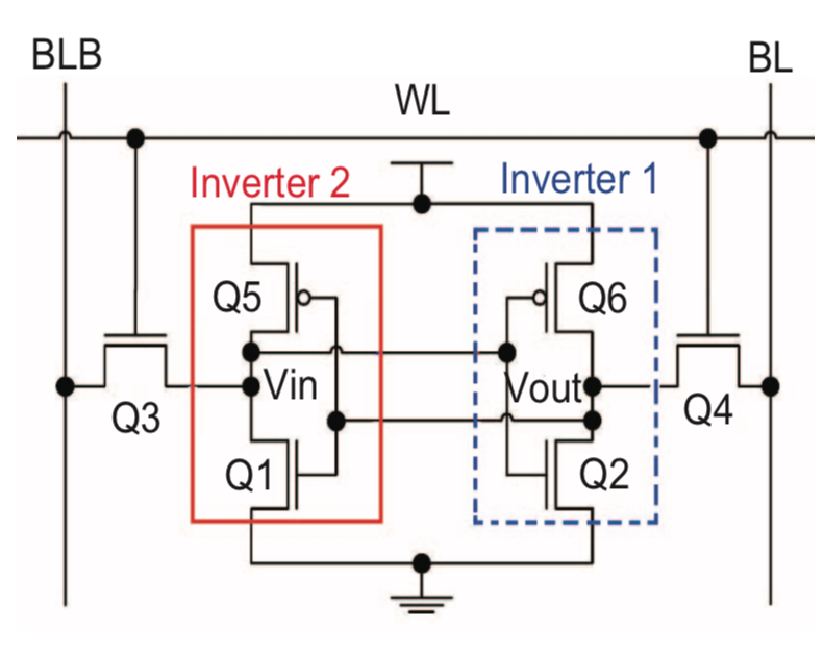
\includegraphics[width={0.5\textwidth}]{images/sram_cell}}
    \caption{A 6-T CMOS SRAM cell \cite{modeling_sram}.}
    \label{fig:sram_cell}
\end{figure}

During manufacturing, there are small differences between each SRAM cell due to process variation which leads to a mismatch in the cell \cite{dargar_2011}. This mismatch also means that the two inverters will always behave distinctly. The mismatch itself does not disturb the normal storage functionality of SRAM cell. Based on this bias, SRAM cells can be classified into three categories as shown below \cite{dargar_2011}:
\begin{enumerate}
\item Non-skewed cell\newline
A non-skewed cell has no preference during its startup due to the impact of process variations does not cause any mismatch between the two inverters. This cell has a heavily fluctuated start-up value depending upon the noise introduced in the system.
\item Partially-skewed cell\newline
A partially-skewed cell has a small mismatch between the inverters which lead to a preference over value '0' or '1' but the cell can flip its value upon variation in external parameters.
\item Fully-skewed cell\newline
A fully-skewed cell is a heavily mismatched SRAM cell in a way that the cell inclined towards value '1' or '0' and has a resistance against external influence/noises.
\end{enumerate}

In ideal SRAM PUF scenario, the utilized SRAM cells should be fully-skewed. Fully-skewed cells lead to a guarantee that the PUF response of a given challenge will have small or no difference even though noises present.


\subsection{Problem: Noise}\label{ch:sram_noise}

Similar to most electronic components, SRAM PUF is also affected by any external influence/noises. These noises will flip unstable bits inside the SRAM PUF. Below are some factors presenting noises:

\begin{itemize}
\item Voltage\newline
The noise introduced by voltage is called power supply noise \cite{wang_tehranipoor_2010}. This noise is related to changes in the delay characteristics of the gate. The changes will occur when there are switchings in the circuit after the device is turned on which increase dynamic power and cause a voltage drop on power lines and voltage increase on ground lines.
\item Temperature\newline
Temperature variation can be introduced by the surroundings or voltage variation. The preference of a cell inside SRAM has a high probability to be affected by temperature \cite{dargar_2011}.
% Temperature affects more than voltage on bit flipping.
\item Crosstalk\newline
Crosstalk appears when a signal transmitted on a circuit introduces unwanted side effects in another circuit. Crosstalk happens due to a tight gap between the SRAM cell (tiny interconnect spacing and width). This event becomes more popular due to wider use of faster-operating speeds and smaller geometries (advancement in nanometer technologies) which lead to higher density. Crosstalk is a major contributor to signal integrity problems in modern designs \cite{wang_tehranipoor_2010}. In addition, higher density in SRAM also influences how environments affect SRAM performance (more prone to voltage and temperature difference) \cite{Abu-Rahma2013}.
\item Aging\newline
Aging is related to changes in the silicon after usage for a long time \cite{rao_mahmoodi_2011}. There are three main effects related to the aging of a circuit; time-dependent dielectric breakdown (TDDB), bias temperature instability (BTI) and hot carrier injection (HCI) \cite{Maricau2013}. TDDB is associated with the creation of a conduction path through the gate transistor structure which causes an increase in power consumption and the circuit delay \cite{impact_mosfet}.
BTI causes a degradation of the transistor threshold voltage \cite{temporal_performance}.
HCI generates a change in the transistor threshold voltage \cite{impact_hot_carriers}. HCI is caused by a high current in the transistor channel injecting charges into the gate oxide during the switching.
\end{itemize}

\subsection{Bit Selection Algorithm} \label{lbl:bit-selection}
As mentioned before, during enrollment, challenge-response pairs are gathered. In SRAM PUF, there are two types of challenges that can be applied to the system. The challenge can be either the whole SRAM memory or specific addresses. If a set of addresses is given as a challenge, an address in there can refer to an address of a byte, a bit, or a sequence of bytes or bits.

If specific addresses of SRAM cells are used for PUF challenge, one of the major steps on using SRAM PUF is looking for stable bits. Stable bits itself refers to fully skewed cells explained before.
Even though the error correction code is present to correct the noise of bit responses, it also has a limitation on how many bits it can correct.
% Since not every SRAM cell is stable, one should take a special caution on deciding which SRAM cell is gonna be the bits to use as PUF input.
Choosing the most stable bits is important to ensure that the PUF result is always the same throughout its lifetime.
Below we present two known algorithms to search for stable bits:
\begin{enumerate}
  \item Neighbor Analysis\newline
The first algorithm is using the rank of total stable neighbors which proposed by Xiao et. al. \cite{xiao_rahman_forte_huang_su_tehranipoor_2014}. They argue that the cells which are “most stable” across environmental conditions are surrounded by more stable cells during enrollment. A stable cell surrounded by more stable cells has a tendency to become more stable because its neighboring cells are likely to experience similar aging stress and operating conditions.
In this algorithm, all the stable cells are given weight according to the number of stable bits surrounding it.
The more stable neighbor cells it has, the higher weight it gets. For example, if a cell is not stable, it is given zero as its score. If it is stable, at least it will get score one. If it only has one stable neighbor on each left and right side, it will get score two as result of an addition of one from being a stable cell and one from having a stable neighbor on both sides. To get score three, it needs to be stable and has two stable neighbors on left and right sides.
After determining the weight of each cell, a heuristic algorithm that greedily chooses cells for the PUF ID/key with weight greater than a threshold is used.

Before the algorithm is performed, one should collect lots of SRAM cells value first. The data should be retrieved in various condition, for example, different voltages, temperatures, and time differences between enrollment.
Afterwards, using the data gathered, the location of all stable bits in SRAM need to be located. A stable bit has to has the same value in all enrollment.
Last, the neighbor analysis algorithm is performed to get the most stable bits in SRAM.

\item Data Remanence Approach\newline
Another bit selection algorithm is by using data remanence of SRAM cell \cite{liu_zhou_tang_parhi_kim_2017}.
There are only two remanence tests involved in this approach: first, writing a value (‘1’ or ‘0’) to the whole memory and second, briefly turning off the power until a few cells flip. The most robust cells are the cells which effortlessly flipped when written with the opposite data. Strong 1's are bits that are flipped fast after 0 is written to its location. On the contrary, if 1 is written to a bit location and the bit flipped fast, it means that the bit is a strong 0.
When using this approach, one should carefully determine the temporal power down time. On one hand, if the temporal power down period is too little, then the data will stay in the previously written state. On the other hand, if the temporal power down time is too lengthy, then the data written in the array will disappear and the SRAM values will go back to its uninitialized state.

A significant advantage using this algorithm compared to the previous one is a much shorter time required to locate stable bits. Using neighbor analysis, there are many SRAM values need to be gathered first which might take hours or days. Locating stable bits from hundreds of data probably also take time as well. If data remanence approach is utilized, there is no need to gather many data. One only need to determine the temporal power down required to get strong bits required. Since usually the temporal down period required is less than 0.5 seconds, this analysis only takes few minutes.
\end{enumerate}

\section{PUF Applications}
In this section, we present three applications which are constructed based on PUF technology. The first application is about generating a key using SRAM PUF, the second one is related to secret key binding based on fuzzy commitment scheme, and the last application is secure key storage using optical PUF and coating PUF.

\subsection{Key Generation using SRAM PUF}

In this section, there are two schemes for key generation presented. Both constructions were built by Hyunho Kang et. al. in 2014. The first construction, shown in Figure \ref{fig:cryptographic_key_generation_old}, utilizes random number generator (RNG). In this example, a key is produced by applying SHA256 hash function on a result of XOR operation between PUF response and a random number. The helper data is generated by XOR-ing PUF response with an encoding of a randomly generated number.
This design was perfected in the second design shown in Figure \ref{fig:cryptographic_key_generation}. In the second design, random number generator was removed to make the construction more efficient without affecting the security. In this design, a key is directly generated based on the PUF response while the helper data is created by XOR-ing the encoding result of PUF-generated key with the PUF response.
Both designs use BCH codes as the error correcting codes with block length ($n$) of 255.

\begin{figure}[tph!]
    \centerline{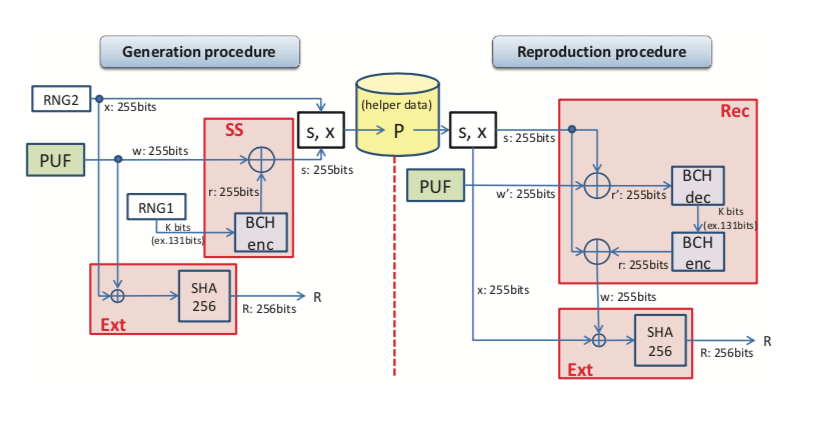
\includegraphics[width={\textwidth}]{images/crypt_key_generation_old}}
    \caption{Implementation diagram using fuzzy extractor (N = 255) \cite{cryptographic_key_generation_old}.}
    \label{fig:cryptographic_key_generation_old}
\end{figure}

\begin{figure}[tph!]
    \centerline{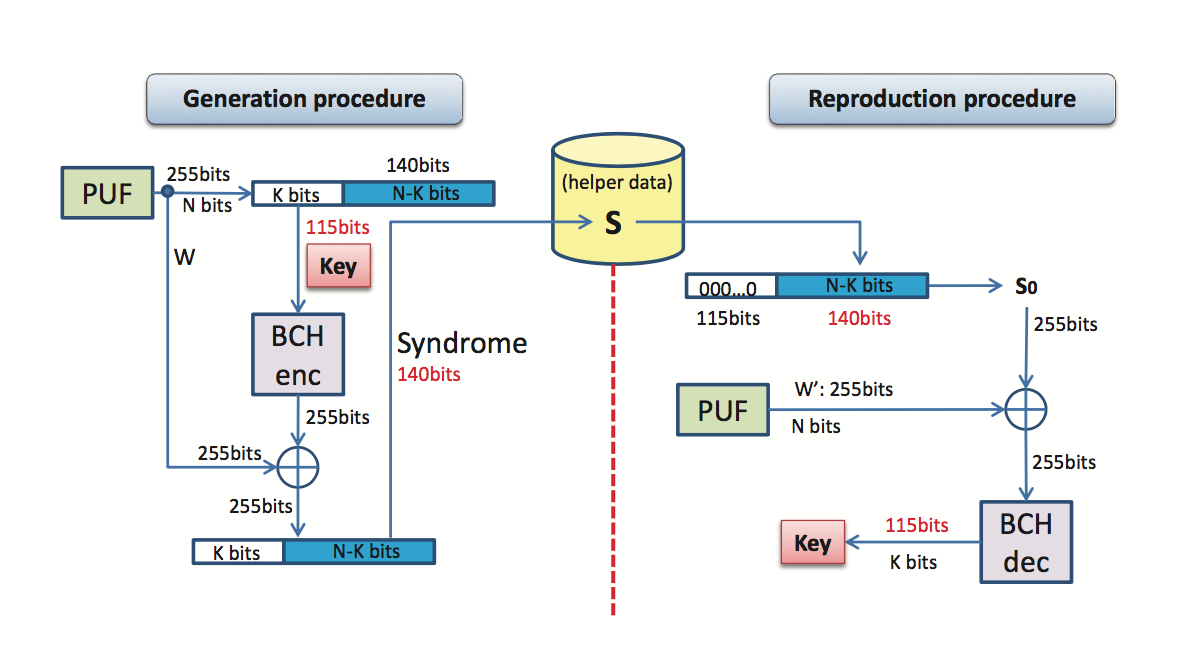
\includegraphics[width={\textwidth}]{images/crypt_key_generation}}
    \caption{Implementation diagram for efficient fuzzy extractor based on the syndrome (N = 255) \cite{cryptographic_key_generation}.}
    \label{fig:cryptographic_key_generation}
\end{figure}

\subsection{Secret Key Binding based on Fuzzy Commitment Scheme}
Fuzzy commitment was originally introduced by Juels and Wattenberg in 1999 \cite{Juels:1999:FCS:319709.319714}. An example of fuzzy commitment application in PUF domain is presented in \cite{8006840}. Figure \ref{fig:fuzzy_commitment} shows the flow of this scheme.
To securely bind the secret, the secret key $S^K$ needs to be chosen first. Afterwards, the secret key is encoded into a binary codeword $C^N$. Then, the helper data $M^N$ is generated by masking (XOR-ing) the codeword with the PUF value $X^N$.
To reconstruct the secret, a noisy version of the codeword $\widetilde{C}^N$ need be calculated by masking the helper data with the noisy version of PUF observation $Y^N$. The secret $\widehat{S}^K$ can be regenerated by decoding the $\widetilde{C}^N$.

\begin{figure}[tph!]
    \centerline{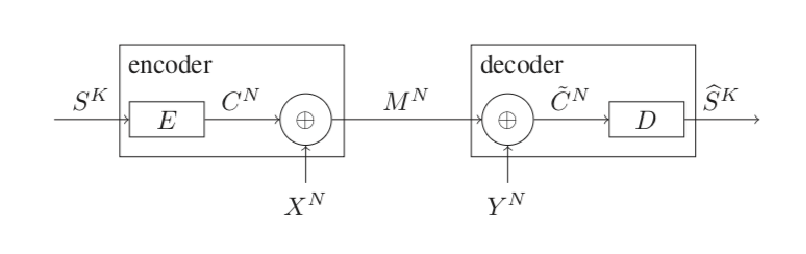
\includegraphics[width={0.8\textwidth}]{images/fuzzy_commitment}}
    \caption{Fuzzy commitment scheme \cite{8006840}.}
    \label{fig:fuzzy_commitment}
\end{figure}


\subsection{Secure Key Storage using Optical PUF and Coating PUF}
In \cite{Skoric2007}, Skoric et. al. present a secure key storage scheme using two extrinsic PUFs; coating PUF and optical PUF. Coating PUF technology is built upon on-chip capacitive quantifications of arbitrary dielectric characteristics of a covering layer which located on top of an IC \cite{10.1007/11894063_29}.  Optical PUF itself consists of a 3-D physical structure containing randomly distributed light-scattering particles that produces a speckle pattern (response) when irradiated with a laser beam \cite{Skoric2007}. This speckle pattern can be considered as the unique fingerprint of the structure. Both PUFs are also considered a strong PUF (has a large CRPs), but optical PUF is considered to be superior than coating PUF due to a much higher number of CRPs and more entropy per response.

% In their scheme, there are two main principle to protect a long term key against physical attacks. First, long term keys should not be stored in non-volatile memory. Second, never let significant portions of the key reside in the volatile memory.
In their scheme, to securely store the key, they proposed to store the long-term key in encrypted form. To access the long-term key, a short-term key extracted from the PUF is required.

\section{Previous Experiments on Off-The-Shelf SRAM PUF}\label{ch:prev_experiments}
There are many experiments related to SRAM PUF which are performed on off-the-shelf SRAM. Most of these experiments are using off-the-shelf SRAM that are embedded in a microcontroller. For example, in \cite{VanHerrewege:2013:DIP:2541806.2512493}, Herrewege et. al. demonstrate a testing of SRAM characteristics on five different microcontrollers; ARM Cortex-A, ARM Cortex-M, Atmel AVR, Microchip PIC16 and Texas Instruments MSP430. They show that not every SRAM embedded in a microcontroller is ideal for an SRAM PUF such as Microchip PIC16F1825. Fortunately, the other microcontroller's SRAMs show an acceptable result to be a PUF candidate (is stable, unique and has enough randomness).
Another example is a work done by Anagnostopoulos et. al. \cite{cryptoeprint:2016:769} in which they present low-temperature data remanence attacks against intrinsic SRAM PUFs, specifically ARM Cortex-M4F LM4F120H5QR microcontroller.

Even though not as many as experiments done on microcontroller's SRAM, there are also some related works that doing the experiments using off-the-shelf SRAM that is not embedded in a specific device. Akhundov in \cite{haji} presents a concept of using SRAM Microchip 23LC1024 as the root-of-trust of his public-key based authentication architecture. He shows the result of HD\textsubscript{intra}, HD\textsubscript{inter} and the distribution of 0's and 1's experiment of Microchip 23LC1024. Unfortunately, the testing was not performed in various condition (different voltage, temperature, and aging effect).
Schrijen and van der Leest in \cite{Schrijen:2012:CAS:2492708.2493033} shows a comparative analysis of seven different SRAMs which manufactured using different technology; Cypress \seqsplit{CY7C15632KV18} (65nm),
Virage HP ASAP SP ULP 32-bit (90nm), Virage HP ASAP SP ULP 64-bit (90nm), Faraday \seqsplit{SHGD130-1760X8X1BM1} (130nm), Virage \seqsplit{asdsrsnfs1p1750x8cm16sw0} (130nm), Cypress \seqsplit{CY7C1041CV33-20ZSX} (150nm), and IDT \seqsplit{71V416S15PHI} (180nm). All of them are tested on the reliability (temperature and voltage variance) and uniqueness (HD\textsubscript{inter} and hamming weight). The results between each SRAM type is different but it can be summarized that all of the tested SRAM memories are suitable as a PUF candidate. Another interesting result from these work is the fact that the most reliable SRAM is achieved by IDT 71V416S15PHI followed by Cypress CY7C1041CV33-20ZSX and Cypress CY7C15632KV18.
Another publication is presented by Holcomb et al. \cite{4674345} where they show start-up measurements from ISSI SRAM, TI microcontrollers, and Intel WISP devices. Unfortunately, the manufacturing technology on these devices is not mentioned.
% Another example is a work done by Zhang et.al in \cite{7459321} where they did an experiment of introducing a novel PUF implementation of the second category that exploits the effect of manufacturing process variations in SRAM read access current
% on SRAM ISSI IS62C256AL to explot Current based PUF Exploiting Random Variations in SRAM Cells

